% DoseRAD2026 final submission — Task: PROTON-MRI (single-task LNCS report, <=11 content pages).
\documentclass{llncs}
\usepackage{amsmath,amssymb,bm,mathtools}
\usepackage{graphicx,booktabs,array}
\usepackage[hidelinks]{hyperref}
\usepackage{tikz}
\usetikzlibrary{arrows.meta,positioning,fit,backgrounds}
\graphicspath{{figs/}}
\newcommand{\opS}{\mathcal{S}}\newcommand{\opD}{\mathcal{D}}\newcommand{\opX}{\mathcal{X}}
\newcommand{\opR}{\mathcal{R}}\newcommand{\opC}{\mathcal{C}}\newcommand{\gam}{\gamma}
\renewcommand{\topfraction}{.95}\renewcommand{\bottomfraction}{.6}
\renewcommand{\textfraction}{.05}\renewcommand{\floatpagefraction}{.75}
\setcounter{topnumber}{3}\setcounter{totalnumber}{5}

\begin{document}

\title{Dose-Aware MR-to-Density Synthesis through a Differentiable Pencil-Beam-Prior Residual
3D U-Net for Proton Dose Prediction on 0.35\,T MRI (DoseRAD2026 Proton-MRI Task)}
\titlerunning{Dose-Aware Synthesis for Proton-MRI Dose Prediction}
\author{Kai Wang \and Meixu Chen \and Rui Yang}
\authorrunning{K. Wang et al.}
\institute{Department of Radiation Oncology, University of Colorado Anschutz Medical Campus,
Aurora, CO, USA\\ \email{\{kai.2.wang,meixu.chen,ray.yang\}@cuanschutz.edu}}

\maketitle

\begin{abstract}
MR-only proton dose prediction is dominated by range: an sCT error that is dosimetrically benign
for photons can displace the Bragg peak. We couple synthesis and dose in one differentiable
pipeline: a classifier--refiner synthesizer maps the 0.35\,T MR \emph{directly to density}
(bypassing the ambiguous HU inversion); differentiable physics channels; skin-entry
water-equivalent path length (WEPL) and a self-contained GPU Hong pencil-beam prior; feed a
residual 3D U-Net; and the synthesizer trains jointly through the physics with the dose loss
plus a WEPL-consistency term that supervises integrated along-beam density, i.e.\ range. Under
5-fold cross-validation on the 75 public patients the system reaches plan
$\gam$1\%/1\,mm\,$=87.4\pm1.9$. A cross-validated real-CT ceiling of $96.1\pm0.9$ isolates the
synthesis cost at $8.7\pm1.9$ points, twice the photon-task cost; and a distal-edge metric
shows it is a range effect: mean distal-$R_{80}$ shift 2.4\,mm (lung 2.8) versus 0.4\,mm on
real CT. On the hidden test set, MR intensity shift was the dominant failure mode;
shift-augmented classification recovered $+3.1$ board gamma. The final full-data submission
scored $\gam$\,=\,79.34, per-beam MAE 0.0247, DVH 5.09 at 188.8\,s per job (later reduced to
110\,s by a batched engine), within the 500\,s gate. We argue the residual gap is limited by the
density information available at 0.35\,T rather than by network capacity.
\keywords{MR-only proton therapy \and synthetic CT \and proton range \and dose-aware synthesis
\and differentiable physics}
\end{abstract}

\section{Introduction}
MR-guided and MR-only proton workflows are emerging for superior soft-tissue targeting and to
avoid CT-to-MR registration error; they require an MR-to-density path, and its accuracy cost is
the central question for their viability. That cost is particle-specific: proton range
integrates density along the whole beam path, so synthesis errors compound into Bragg-peak
shifts, whereas photon dose is density-tolerant. Existing MR-only proton dosimetry synthesizes a
CT (or stopping power) under an \emph{image}
objective~\cite{mriproton,rsp,liver,ganbrain,uncert,dect} and computes dose separately. We
instead make the synthesis \emph{dose-aware}: an analytical, differentiable physics operator
$\opC$ (skin-entry WEPL, a GPU pencil-beam prior~\cite{hong} supplying $\sim$95\% of the dose,
lateral distance, energy) feeds a residual 3D U-Net $\opD_\theta$, and the MR-to-density
synthesizer trains \emph{through} $\opC$ with the dose loss. Range receives two dedicated
signals: the synthesizer outputs \emph{density directly} (no HU round-trip), and a
WEPL-consistency loss supervises the integrated along-beam density explicitly. This report
details the Proton-MRI system and quantifies; via a cross-validated real-CT ceiling and a
distal-edge metric, exactly how much accuracy MR-only proton calculation costs and why; the
same framework serves our submissions to all four DoseRAD2026 tasks.

\begin{figure}[t]\centering
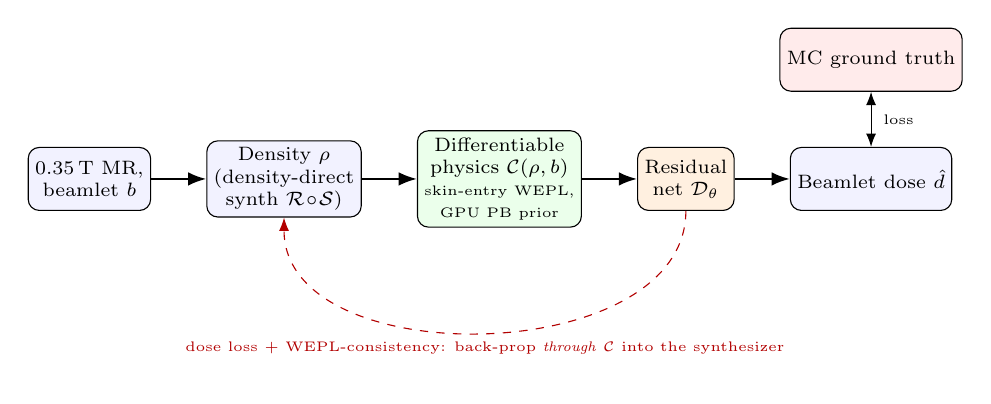
\begin{tikzpicture}[
 node distance=6mm and 7mm, >=Latex, font=\scriptsize,
 box/.style={draw, rounded corners, align=center, minimum height=8mm, inner sep=2.5pt, fill=blue!5},
 phys/.style={box, fill=green!8}, net/.style={box, fill=orange!12},
 every edge/.style={draw, ->, thick}]
\node[box] (img) {0.35\,T MR,\\ beamlet $b$};
\node[box, right=of img] (dens) {Density $\rho$\\ (density-direct\\ synth $\opR\!\circ\!\opS$)};
\node[phys, right=of dens] (chan) {Differentiable\\ physics $\opC(\rho,b)$\\ \tiny skin-entry WEPL,\\ \tiny GPU PB prior};
\node[net, right=of chan] (net) {Residual\\ net $\opD_\theta$};
\node[box, right=of net] (dose) {Beamlet dose $\hat d$};
\node[box, above=7mm of dose, fill=red!8] (mc) {MC ground truth};
\draw (img) edge (dens) (dens) edge (chan) (chan) edge (net) (net) edge (dose);
\draw[<->] (dose) -- (mc) node[midway,right=1pt]{\tiny loss};
\draw[->, dashed, red!70!black] (net.south) to[out=-90,in=-90] node[midway,below,align=center]
 {\tiny dose loss $+$ WEPL-consistency: back-prop \emph{through} $\opC$ into the synthesizer} (dens.south);
\end{tikzpicture}
\caption{Dose-aware MR-only proton pipeline: density-direct synthesis trained jointly through
the differentiable physics with the dose loss and a WEPL-consistency (range)
term.}\label{fig:framework}
\end{figure}

\section{Methods}
\subsection{Data}
Official DoseRAD2026 training set~\cite{challenge} (75 patients: 39 thorax, 36 abdomen;
SynthRAD2025 cohort~\cite{synthrad}): per patient a co-registered 0.35\,T MR (ViewRay MRIdian,
bSSFP) and planning CT, beam parameters, and per-beamlet MC dose-to-medium
(matRad~\cite{matrad}) on the native $1{\times}1{\times}3$\,mm grid; several hundred to
$\sim$a thousand beamlets per patient. The MRI-task ground truth is the CT-computed MC dose
mapped onto the co-registered MR, so the real-CT dose is the achievable target (the framing of
our ceiling analysis, Sec.~3.3). The sCT refiner additionally uses 166 field-matched 0.35\,T
MR--CT pairs from the public SynthRAD2025 pool (disjoint from validation); no other external
data. Development: 5-fold CV over all 75; \textbf{the final submission is retrained on all 75}.

\subsection{Model}
\textbf{Synthesizer} $\opX=\opR\circ\opS$: whole-image classifier $\opS$
(air/lung/soft/bone $\to$ bulk coarse CT) and refiner $\opR$; for protons the refiner outputs
\emph{relative density directly} (clamped to $[0,\rho_{\max}]$); the HU$\to$density calibration
is many-to-one and its inversion is an unnecessary, error-amplifying step between the network
and the physics. The 2\,mm synthesis is resampled to the native $1{\times}1{\times}3$\,mm dose
grid by a differentiable physical-coordinate grid sample, so dose gradients reach the 2\,mm
synthesizer. \textbf{Physics} $\opC$: five differentiable channels per beamlet; density/RSP,
skin-entry WEPL (per-voxel, corrected scheme; the naive beam's-eye-view fan over-counts
systematically), the GPU Hong pencil-beam prior ($r{=}0.995$ vs.\ pyRadPlan, $\sim$40\,ms/beamlet,
no planning-system dependency at inference), lateral distance, energy. \textbf{Dose network}
$\opD_\theta$: DoseUNet3D (base 48, ASPP bottleneck, Softplus head, FiLM conditioning),
warm-started from Proton-CT. Figure~\ref{fig:chain} shows the deployed chain; synthesis and
its dosimetric consequence in one figure.

\begin{figure}[t]\centering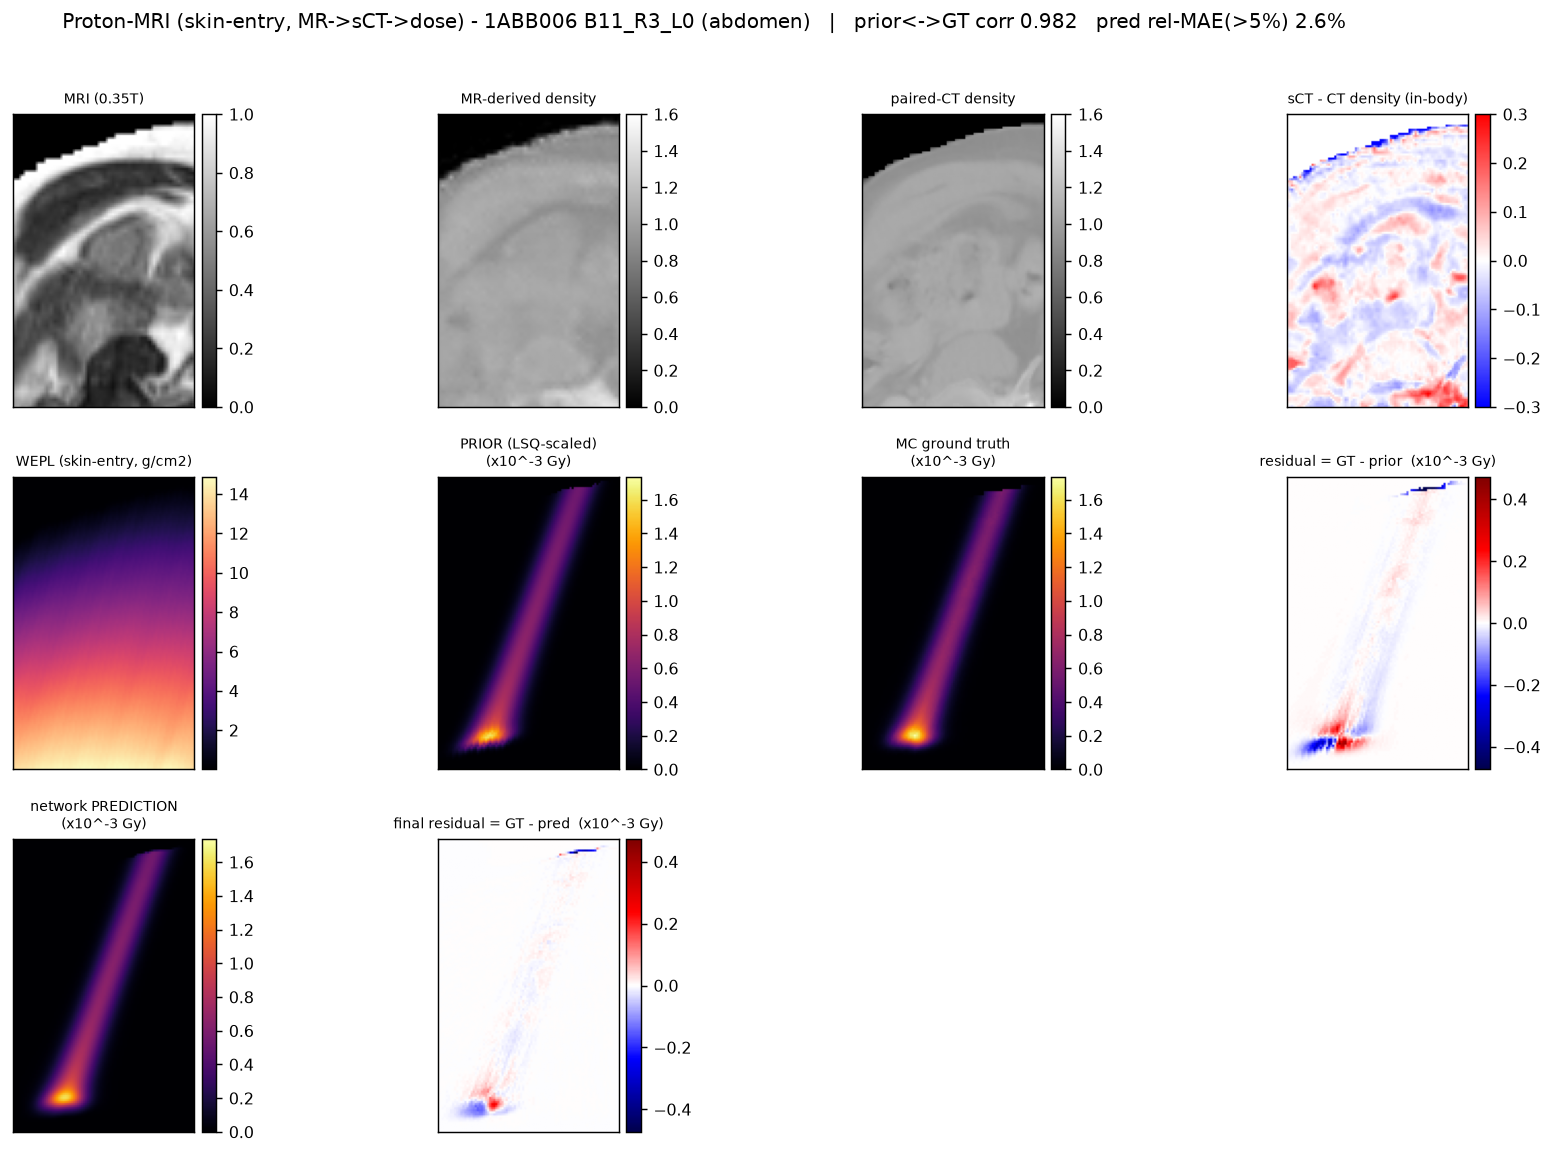
\includegraphics[width=\linewidth]{figS_residual_protonmri_abdomen.png}
\caption{Deployed Proton-MRI chain (abdomen, 1ABB006). Row 1: synthesis ; MR (0.35\,T) $\to$
MR-derived density $\to$ paired-CT density $\to$ in-body density residual. Remaining panels:
WEPL on the synthetic density $\to$ pencil-beam prior (Gy) $\to$ MC ground truth $\to$ residual
(GT$-$prior) $\to$ prediction $\to$ final residual (GT$-$pred).}\label{fig:chain}\end{figure}

\begin{figure}[t]\centering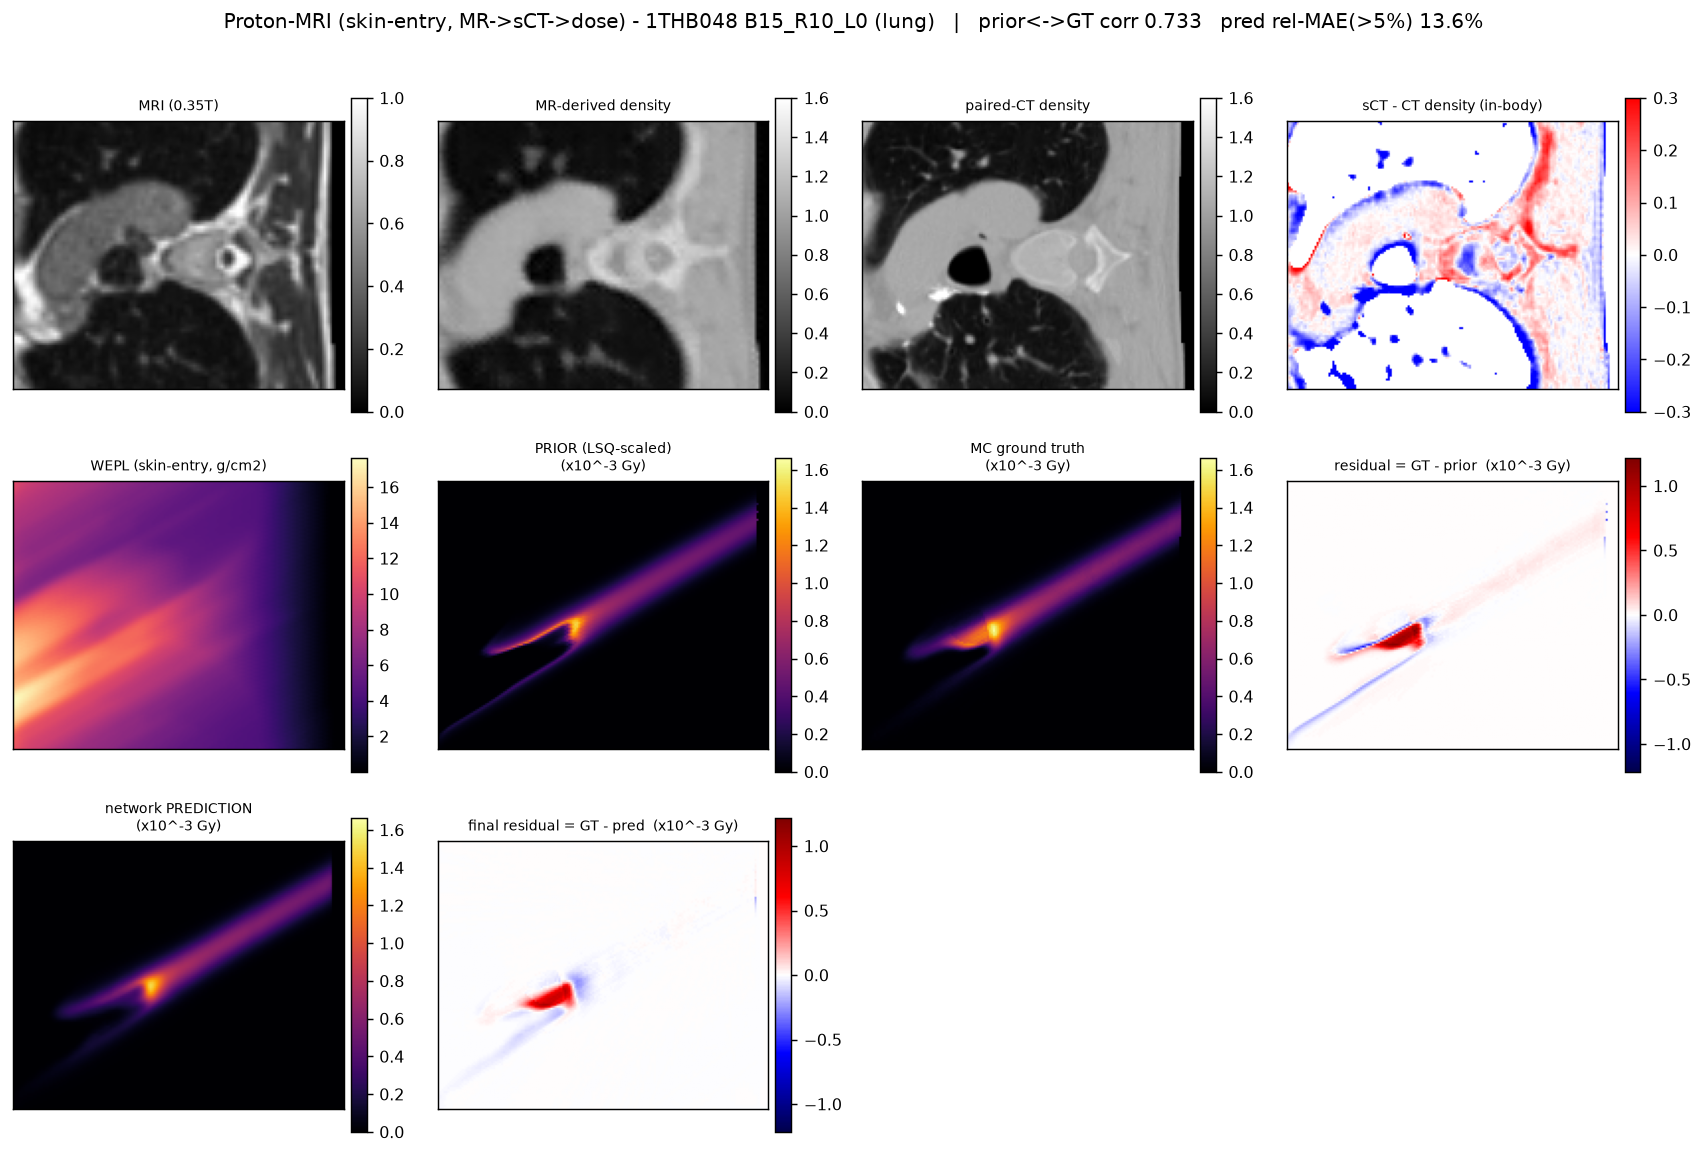
\includegraphics[width=\linewidth]{figS_residual_protonmri_lung.png}
\caption{As Fig.~\ref{fig:chain}, lung case: the largest synthesis-induced range errors
concentrate in lung, where 0.35\,T MR carries the least density
information.}\label{fig:chainlung}\end{figure}

\subsection{Training}
Stage 1: classifier/refiner pretraining (refiner also on the 166 field-matched pairs); dose
network warm-started from Proton-CT. Stage 2 (dose-aware): refiner and dose network train
jointly end-to-end (15--20k steps), the dose loss back-propagating through the WEPL and prior
channels into the synthesizer, with two proton-specific additions: the \emph{density-direct}
output head and the \emph{WEPL-consistency loss}
$\lambda_w\lVert\mathrm{WEPL}(\hat\rho)-\mathrm{WEPL}(\rho_{\rm CT})\rVert_1$, which supervises
the range-determining integral directly and is more localized than the dose loss. A
region-weighted sCT anchor regularizes synthesis. \textbf{Hidden-test robustness:} leaderboard
probes identified MR \emph{intensity shift} as the dominant held-out failure mode, with the
shared tissue classifier the main culprit; the deployed classifier is retrained with strong
intensity-shift augmentation (recovering $+3.1$ board gamma), and, a deployment-critical
detail; it must run \emph{sliding-window} at the native grid: whole-image classifier inference
collapsed lung on some test grids (single-patient gamma 90$\to$48) before we gated for it.
Reproducibility: fixed seeds, YAML configs, EMA checkpoints; code and weights to be open-sourced
(Sec.~6).

\subsection{Evaluation}
Internal: plan-level local $\gam$~\cite{gamma} (pymedphys, 1\%/1\,mm, $\ge$10\% Rx cutoff,
byte-identical to the vendored official code), per-beamlet masked MAE, official IDD and
stratified-MAE reimplementations; frozen 16-patient held-out cohort gating every deployment
change. Mechanistic probes: the \emph{real-CT ceiling} (real CT substituted for the synthesis,
patient-matched) and a \emph{distal-edge range metric}; the absolute shift of the distal
$R_{80}$/$R_{90}$ along the beamlet axis on the 100 highest-dose beamlets per patient; because
an aggregate gamma under-reports exactly the distal-range failure mode that matters for protons.
Runtime: official $T=t_{\rm fix}+N\cdot t_{\rm dose\,map}$, gate 500\,s/job, double-weighted.

\section{Results}
\subsection{Accuracy: cross-validated and hidden-test}
Per-fold CV $\gam$1/1: 84.0/88.9/88.9/86.7/88.6 (mean $87.4\pm1.9$). Development fold ($n=16$):
$\gam$1/1 $=83.7\pm6.8$ (abdomen 88.8, lung 78.6), $\gam$2/2 $=95.4$, $\gam$3/3 $=98.4$;
per-beamlet masked MAE $2.02\pm0.49$\%. Table~\ref{tab:res} adds the hidden-test metrics. As on
the photon-MRI task, the CV-to-hidden-test drop is dominated by MR intensity shift; the
shift-augmented classifier recovered $+3.1$ board gamma over the unaugmented deployment and is
part of the final submission.

\begin{table}[t]\centering
\caption{Proton-MRI results. CV: 5-fold over the 75 public patients. Hidden test: official
metrics of the final full-data submission (August 2026). Gate: 500\,s/job.}\label{tab:res}
\begin{tabular}{@{}lc@{}}\toprule
Metric & Value\\\midrule
CV plan $\gam$1\%/1\,mm (5-fold) & $87.4\pm1.9$\\
CV real-CT ceiling / synthesis cost & $96.1\pm0.9$ / $8.7\pm1.9$\\
Hidden-test per-beam masked MAE & $0.0247\pm0.0104$\\
Hidden-test IDD curve distance & $0.0233\pm0.0101$\\
Hidden-test stratified plan MAE & $0.0253\pm0.0098$\\
Hidden-test plan $\gam$1\%/1\,mm & $79.34\pm12.23$\\
Hidden-test DVH clinical score & $5.09\pm5.57$\\
Hidden-test runtime per job & 188.8\,s (batched engine: 110\,s)\\\bottomrule
\end{tabular}\end{table}

\subsection{The synthesis cost is a range effect}
Re-running the trained pipeline of every fold with the \emph{real} CT substituted for the
synthesis gives a ceiling of $96.1\pm0.9$, closely reproducing our Proton-CT task accuracy
($96.7\pm1.0$), so fed a real CT the MR pipeline behaves like the CT pipeline, and the deficit
is genuinely a synthesis cost: $8.7\pm1.9$ points patient-matched, versus $4.7\pm1.4$ on the
photon-MRI task ($\sim$1.9$\times$; on the development fold the paired contrast is
$-13.3\pm6.1$ vs.\ $-5.0\pm5.0$, $p\ll0.001$, with \emph{every} patient losing under proton;
Fig.~\ref{fig:cost}). The distal-edge metric (Table~\ref{tab:range}) identifies the mechanism:
the mean distal-$R_{80}$ shift is $2.39\pm1.04$\,mm on the synthesis versus $0.38\pm0.20$\,mm on
real CT, a $\sim$6$\times$ range error, concentrated in lung, exactly the failure mode an
aggregate gamma under-reports.

\begin{table}[h]\centering
\caption{Distal-edge range accuracy: absolute shift of the distal $R_{80}$/$R_{90}$ (mm) along
the beamlet axis, 100 highest-dose beamlets per patient (development fold, 8 abdomen / 8
lung).}\label{tab:range}
\begin{tabular}{@{}llcc@{}}\toprule
Input & Site & $R_{80}$ shift (mm) & $R_{90}$ shift (mm)\\\midrule
real CT  & abdomen & $0.25\pm0.08$ & $0.25\pm0.07$\\
real CT  & lung    & $0.51\pm0.20$ & $0.47\pm0.15$\\
real CT  & all     & $\mathbf{0.38\pm0.20}$ & $0.36\pm0.16$\\
MR synthesis & abdomen & $1.94\pm0.53$ & $1.94\pm0.52$\\
MR synthesis & lung    & $2.84\pm1.25$ & $2.59\pm1.17$\\
MR synthesis & all     & $\mathbf{2.39\pm1.04}$ & $2.26\pm0.93$\\\bottomrule
\end{tabular}\end{table}

\begin{figure}[t]\centering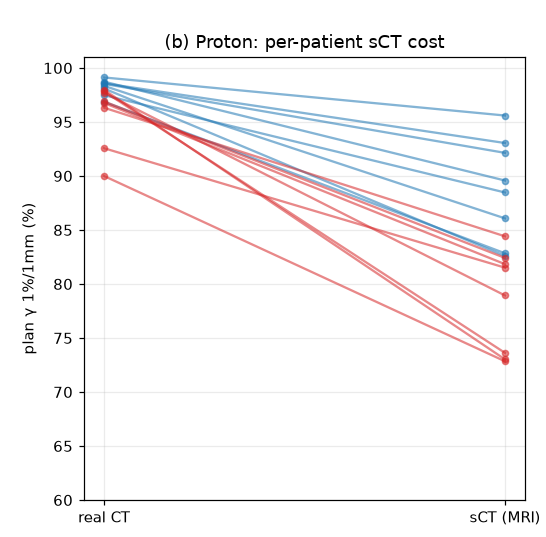
\includegraphics[width=.6\linewidth]{fig_sctcost_protonmri.png}
\caption{Per-patient synthesis cost on this task (real CT vs.\ MR-derived density input, development fold; blue abdomen, red lung): \emph{every} patient loses accuracy, lung most; proton range integrates density. The corresponding photon cost is $\sim$2$\times$ smaller (see text).}\label{fig:cost}\end{figure}

\subsection{Method-level ablations are small; the particle contrast is the robust result}
Per-patient paired tests on the development fold (Table~\ref{tab:abl}): the WEPL-consistency
loss ($+0.37$, $p{=}0.35$) and density-direct synthesis ($+0.36$, $p{=}0.25$) are consistent,
abdomen-driven trends, exactly where MR-recoverable density lives; but individually within
noise at $n{=}16$, and both are null on the photon-MRI task by design. We therefore rest the
interpretive weight not on these deltas but on the highly significant particle contrast (every
patient loses under proton synthesis, $p\ll0.001$) and on the cross-validated accuracy. Bone/air
segmentation fixes and loss re-weighting toward bone likewise did not move gamma
($p{=}0.57$), consistent with our diagnosis that the residual synthesis error is spatially
unstructured soft-tissue error plus lung, not a fixable segmentation artifact.

\begin{table}[h]\centering
\caption{Proton-MRI method ablations, per-patient paired tests (development fold, $n=16$,
$\gam$1\%/1\,mm).}\label{tab:abl}
\begin{tabular}{@{}lccc@{}}\toprule
Comparison & $\Delta\gam$ (mean$\pm$SD) & W/T/L & Wilcoxon $p$\\\midrule
$+$WEPL-consistency vs dose-aware baseline & $+0.37\pm1.22$ & 10/0/6 & 0.35\\
$+$density-direct vs $+$WEPL & $+0.36\pm0.84$ & 8/1/7 & 0.25\\
(ref) proton synthesis cost & $\bm{-13.3\pm6.1}$ & 16/0/0 & $\bm{\ll0.001}$\\\bottomrule
\end{tabular}\end{table}

\subsection{Decomposing the synthesis error, and what did not fix it}
Where does the $8.7$-point cost live? Direct decomposition of the deployed synthesis against the
paired CT gives three components. \emph{Range}: the WEPL-relevant integrated error corresponds
to $\sim$3\,mm of range uncertainty where $\sim$1\,mm would be needed for CT-grade gamma; the
dominant term, matching the $R_{80}$ analysis. \emph{Soft tissue}: $\sim$41\% of in-body
density error sits in soft tissue and is spatially unstructured (near-random residual after the
refiner), i.e.\ not attributable to any segmentable class. \emph{Interfaces}: bone/air
boundary errors exist but are minor contributors. This decomposition predicted, correctly, that
several plausible fixes would fail, and we report them as tested negatives: bone-weighted
anchor losses ($+0.05\,\gam$, $p{=}0.57$); better lung segmentation (TotalSegmentator-MRI mask,
no gamma gain); retraining the synthesis at the native $1{\times}1{\times}3$\,mm grid (failed
our no-loss gate; the apparent ``2\,mm bottleneck'' was illusory); and whole-image synthesis
variants (on par, not better). What \emph{did} move the board was none of the above but the
intensity-shift-augmented classifier ($+3.1$; Sec.~2.3): generalization, not in-domain
synthesis fidelity, was the binding constraint. A methodological lesson underlying all of this:
in-sample validation misled us early ($\gam\,96$-level in-sample vs.\ 76 held-out on our first
board submission), and every conclusion above is from held-out or leaderboard measurement.


\begin{figure}[t]\centering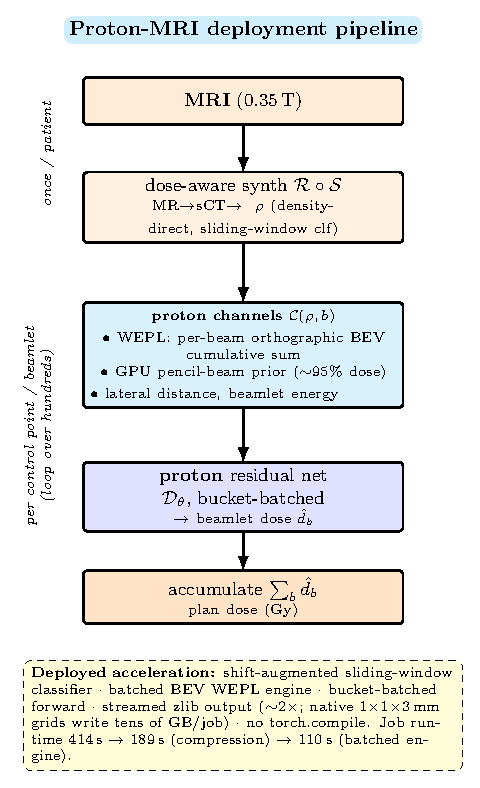
\includegraphics[width=.55\linewidth]{fig_deploy_protonmri.pdf}
\caption{The deployed Proton-MRI container: per patient, the density stage runs once; the
differentiable-channels $\to$ residual-net loop runs per control point/beamlet. The callout
lists the deployed acceleration measures and their measured effects.}\label{fig:deploy}\end{figure}

\subsection{Runtime engineering}
Proton-MRI shares the Proton-CT deployment stack and adds the synthesis stage (classifier
sliding-window $+$ refiner, $\sim$2\,s per source image). The first submitted engine reduced
runtime from 414\,s to 188.8\,s per job chiefly through streamed zlib-compressed output with a
writer pool (proton jobs write tens of GB on the native grid and are write-bound without
overlap). The batched engine then collapsed per-beam WEPL to one orthographic beam's-eye-view
cumulative sum (beamlet rays within a beam are exactly parallel; $388\times$ on the WEPL stage),
bucket-batched the network forward (exact by same-shape bucketing), and streamed per-beam
chunks: measured 110\,s per job on the platform at unchanged accuracy. A platform finding worth
reporting: the evaluation service starts a fresh process per job, so \texttt{torch.compile}
pays a $\sim$50\,s tax per job and recompiles on each new patient grid (one measured multi-grid
job: 238\,s compiled vs.\ 110\,s eager); the proton engines therefore ship without compile.



\begin{figure}[t]\centering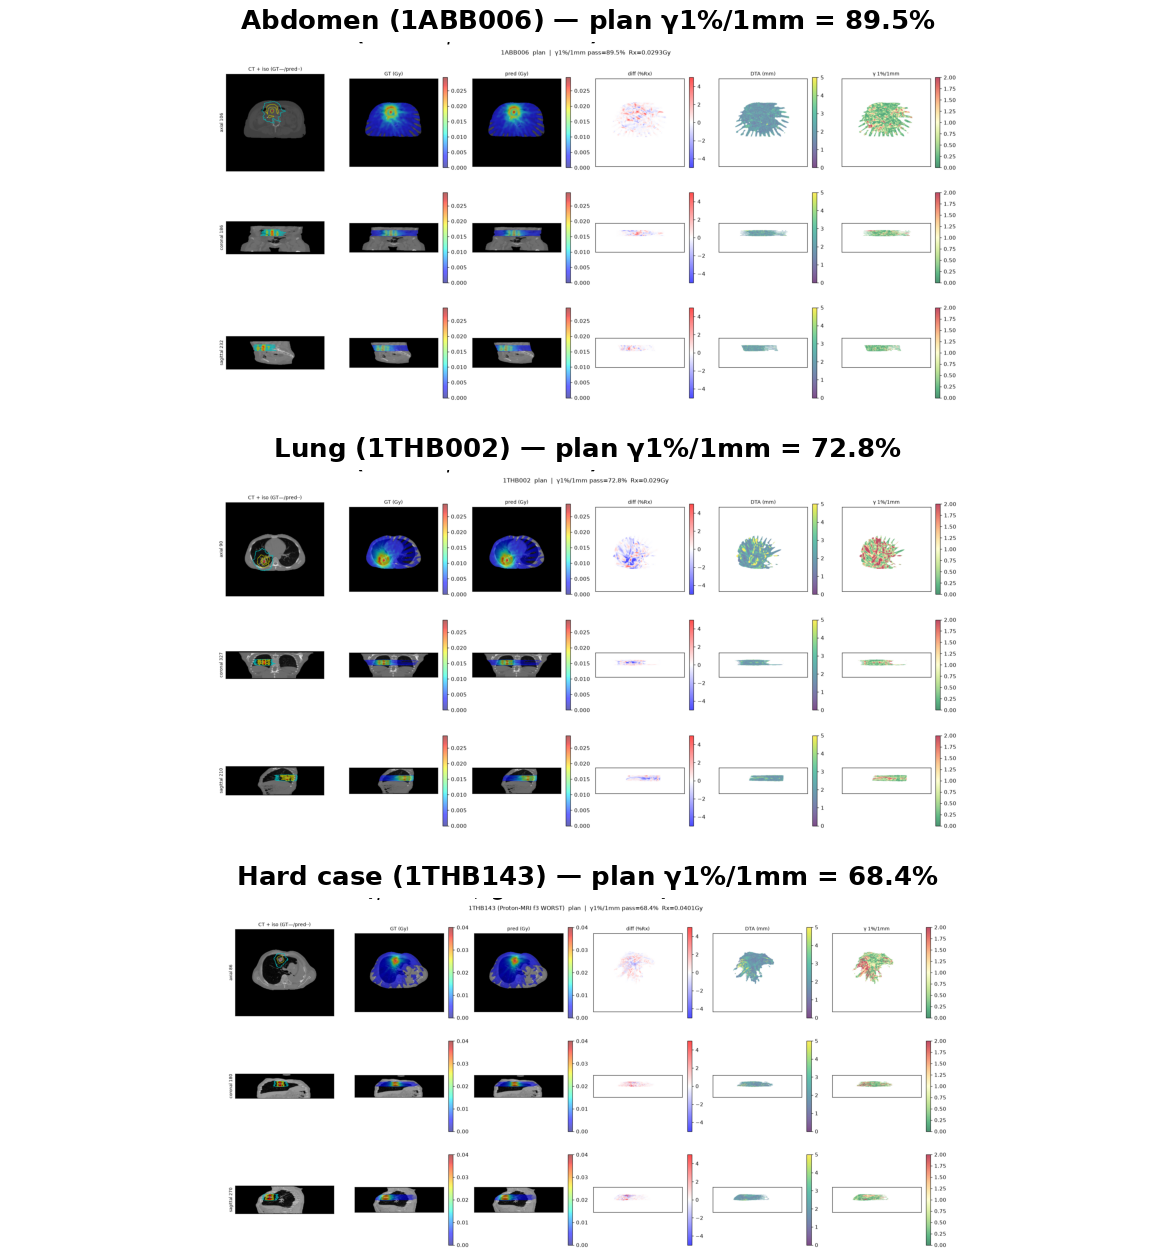
\includegraphics[width=.92\linewidth]{fig_qual_protonmri.png}
\caption{Qualitative Proton-MRI results on three cases spanning the difficulty range: abdomen (1ABB006, plan $\gam$1/1 $=89.5$), lung (1THB002, $72.8$), and the geometrically hard case 1THB143 ($68.4$; the worst patient in all four challenge tasks simultaneously, yet largely passing at 3\%/3\,mm: small-magnitude errors at steep lung--tissue interfaces). Columns: image with GT (solid) and predicted (dashed) isodose, MC dose, predicted dose, difference, distance-to-agreement, local $\gam$1\%/1\,mm.}\label{fig:qual}\end{figure}

\section{Discussion}
The central quantitative result of this task is an accuracy cost: MR-only proton dose prediction
at 0.35\,T costs $8.7\pm1.9$ gamma points against the same pipeline on real CT, it is a
\emph{range} effect (6$\times$ larger distal-$R_{80}$ shift, concentrated in lung), and it is
roughly twice the corresponding photon cost. Dose-aware synthesis, density-direct output and
WEPL supervision each push in the right direction but do not close it; nor did better
segmentation or bone-weighted losses. We conclude the residual gap is limited primarily by the
density information available in 0.35\,T bSSFP MR (and by cohort size), not by network
capacity, which locates the promising levers at higher field strength, larger MR-only cohorts,
and possibly sCT-free direct MR-to-dose learning, rather than at architecture.
\textbf{Limitations and generalizability.} Single benchmark, single scanner; the hidden-test
intensity shift is a preview of cross-device shift, and our shift-augmented classifier recovers
only part of it. Ground truth is CT-computed dose mapped to the MR, so registration residuals
are label noise. Method-level ablations are single-fold ($n{=}16$) and individually
non-significant; the particle contrast and the CV accuracy carry the conclusions. For clinical
MR-only proton planning, the ceiling analysis offers a usable decision tool: it measures,
per-site, how much accuracy the MR-to-density path costs against a CT-based plan.

\emph{Why an intermediate density image?} The density map is the interface to the
physics: WEPL and the pencil-beam prior consume it, and they supply $\sim$95\% of the dose
signal that a direct MR-to-dose network would need to relearn from 75 patients. The synthesizer
is partially transferred (166 field-matched SynthRAD2025 pairs pretrain the refiner). Note also
that the dose-aware density genuinely diverges from an imaging-optimized sCT: optimized through
the dose loss and the WEPL-consistency term, it trades image fidelity for range fidelity, and
should not be reused as a diagnostic image. Whether an sCT-free direct MR-to-dose model can
match this pipeline is untested here and is our first future-work item.

\textbf{Future work.} Our error decomposition dictates the roadmap. (i) \emph{sCT-free direct
MR-to-dose}: since the soft-tissue residual is unstructured and every synthesis-side fix we
tested was flat, the most promising escape is to stop forcing the information through an
explicit density image: learn dose (or a dose correction to a provisional-density prior)
directly from the MR, keeping the differentiable physics as scaffolding. (ii) \emph{Range-first
data}: higher field strength and larger MR-only cohorts attack the $\sim$3\,mm range error at
its information source; UTE/ZTE or multi-contrast acquisitions that see bone and lung structure
are the acquisition-side lever. (iii) \emph{Uncertainty-aware planning integration}: the
per-voxel synthesis uncertainty our anchor framework already estimates could feed robust-plan
optimization~\cite{uncert} rather than being discarded, turning a known 2--3\,mm range
uncertainty into margins instead of errors. (iv) \emph{Generalization as a first-class
objective}: the intensity-shift result (the single largest board improvement of our
campaign) suggests routine adversarial/physics-based MR appearance augmentation and
held-out-center validation should precede any further in-domain accuracy work.

\section{Author Contributions (CRediT)}
\textbf{Kai Wang:} Conceptualization, Methodology, Software, Validation, Formal analysis,
Investigation, Data curation, Writing -- original draft, Visualization.
\textbf{Meixu Chen:} Software (deployment and runtime optimization), Investigation
(acceleration study), Validation, Writing -- review \& editing.
\textbf{Rui Yang:} Conceptualization, Methodology, Writing -- review \& editing, Supervision.

\section{Other Information}
\textbf{Funding:} No external funding was received for this work.
\textbf{Collaborators:} None beyond the listed authors.
\textbf{Writing assistance:} Large-language-model assistance (Claude, Anthropic) was used in drafting and editing the text of this report; all methods, experiments, analyses and conclusions are the authors' own.
\textbf{Code availability:} The full implementation (models, differentiable physics operators,
the GPU pencil-beam prior, deployment containers, and weights) will be released open-source at
\url{https://github.com/wangkaiwan/PhyPriorNet} before the challenge deadline (2026-10-01).

\clearpage
\begin{thebibliography}{9}\small
\bibitem{mriproton} Tian, L., et al.: MRI-based proton dose calculation for pelvic tumors using
deep learning. Phys. Med. Biol. \textbf{71}, 045003 (2026)
\bibitem{rsp} Gao, Y., et al.: MRI-only based material mass density and relative stopping power
estimation via deep learning for proton therapy. Sci. Rep. \textbf{14}, 11166 (2024)
\bibitem{liver} Liu, Y., et al.: MRI-based treatment planning for proton radiotherapy: dosimetric
validation of a deep-learning liver synthetic-CT method. Phys. Med. Biol. \textbf{64}, 145015 (2019)
\bibitem{ganbrain} Kazemifar, S., et al.: Dosimetric evaluation of synthetic CT generated with
GANs for MRI-only proton therapy planning of brain tumors. J. Appl. Clin. Med. Phys.
\textbf{21}(5), 76--86 (2020)
\bibitem{uncert} Li, X., et al.: Uncertainty-aware MR-based CT synthesis for robust proton therapy
planning of brain tumour. Radiother. Oncol. \textbf{189}, 109902 (2023)
\bibitem{dect} Liu, R., et al.: Synthetic dual-energy CT for MRI-only based proton therapy
treatment planning using label-GAN. Phys. Med. Biol. \textbf{66}, 065014 (2021)
\bibitem{hong} Hong, L., et al.: A pencil beam algorithm for proton dose calculations. Phys. Med.
Biol. \textbf{41}, 1305--1330 (1996)
\bibitem{gamma} Low, D.A., Harms, W.B., Mutic, S., Purdy, J.A.: A technique for the quantitative
evaluation of dose distributions. Med. Phys. \textbf{25}, 656--661 (1998)
\bibitem{matrad} Wieser, H.P., et al.: Development of the open-source dose calculation and
optimization toolkit matRad. Med. Phys. \textbf{44}, 2556--2568 (2017)
\bibitem{challenge} DoseRAD2026 Grand Challenge, \url{https://doserad2026.grand-challenge.org} (2026)
\bibitem{synthrad} Thummerer, A., et al.: SynthRAD2025 Grand Challenge dataset: generating
synthetic CTs for radiotherapy. Med. Phys. (2025)
\end{thebibliography}

\end{document}
